\documentclass[a4paper, 12pt]{article}%тип документа

%отступы
\usepackage[left=1.5cm,right=1cm,top=2cm,bottom=3cm,bindingoffset=0cm]{geometry}
\setlength{\parindent}{5ex}

%Русский язык
\usepackage[T2A]{fontenc} %кодировка
\usepackage[utf8]{inputenc} %кодировка исходного кода
\usepackage[english,russian]{babel} %локализация и переносы

%Вставка картинок
\usepackage{graphicx}
\graphicspath{{pictures/}}
\DeclareGraphicsExtensions{.pdf,.png,.jpg,}
\usepackage{wrapfig}

%Графики
\usepackage{pgfplots}
\pgfplotsset{compat=1.9}

%Математика
\usepackage{amsmath, amsfonts, amssymb, amsthm, mathtools}

%Таблицы
\usepackage{longtable} 
\usepackage{float}

%Римские цифры
\newcommand{\RomanNumeralCaps}[1]{\uppercase\expandafter{\romannumeral#1}}

\usepackage{multirow}

\begin{document}
	
\textbf{Задание №1: Матрица направляющих косинусов углов Эйлера}\\ 

	\begin{eqnarray*}
	 &C \cdot B \cdot A = \left(\begin{array}{ccc}1 & 0 & 0 \\ 0 & \cos \alpha & -\sin \alpha \\ 0 & \sin \alpha & \cos \alpha\end{array}\right)\left(\begin{array}{ccc}\cos \beta & 0 & \sin \beta \\ 0 & 1 & 0 \\ -\sin \beta & 0 & \cos \beta\end{array}\right)\left(\begin{array}{ccc}\cos \gamma & -\sin \gamma & 0 \\ \sin \gamma & \cos \gamma & 0 \\ 0 & 0 & 1\end{array}\right) =   &\\ &=\left(\begin{array}{ccc}\cos \beta \cos \gamma & -\sin \gamma \cos \beta & \sin \beta \\ \sin \alpha \sin \beta \cos \gamma+\sin \gamma \cos \alpha & -\sin \alpha \sin \beta \sin \gamma+\cos \alpha \cos \gamma & -\sin \alpha \cos \beta \\ \sin \alpha \sin \gamma-\sin \beta \cos \alpha \cos \gamma & \sin \alpha \cos \gamma+\sin \beta \sin \gamma \cos \alpha & \cos \alpha \cos \beta\end{array}\right) &
	\end{eqnarray*} \\
	
	
	\textbf{Задание №2: Кинематические и динамические уравнения Эйлера }\\ 
	

	$\begin{cases}
		
		\begin{array}{l}\omega_{\xi}=\dot{\varphi} \sin \theta \sin \psi+\dot{\theta} \cos \psi \\ \omega_\eta=\dot{\varphi} \sin \theta \cos \psi-\dot{\theta} \sin \psi \\ \omega_\zeta=\dot{\psi}+\dot{\varphi} \cos \theta\end{array} \\
		\left[\begin{array}{ccc}I_{\xi} & 0 & 0 \\ 0 & I_{\eta} & 0 \\ 0 & 0 & I_{\zeta}\end{array}\right]\left[\begin{array}{l}\dot{\omega}_{\xi} \\ \dot{\omega}_\eta \\ \dot{\omega}_{\zeta}\end{array}\right]+\left[\begin{array}{l}\omega_{\xi} \\ \omega_\eta \\ \omega_{\zeta}\end{array}\right] \times\left(\left[\begin{array}{ccc}I_{\xi} & 0 & 0 \\ 0 & I_{\eta} & 0 \\ 0 & 0 & I_\zeta\end{array}\right]\left[\begin{array}{l}\omega_{\xi} \\ \omega_\eta \\ \omega_{\zeta}\end{array}\right]\right)=\left[\begin{array}{l}M_1 \\ M_2 \\ M_3\end{array}\right]
	\end{cases}$
	
\addvspace{20pt}


	$
	\begin{cases}
		\begin{array}{l}\omega_{\xi}=\dot{\varphi} \sin \theta \sin \psi+\dot{\theta} \cos \psi \\ \omega_\eta=\dot{\varphi} \sin \theta \cos \psi-\dot{\theta} \sin \psi \\ \omega_\zeta=\dot{\psi}+\dot{\varphi} \cos \theta\end{array} \\
		\begin{array}{l}\dot\omega_{\xi} = \frac{M_1 -\omega_{\zeta}\omega_{\eta}(I_{\zeta} - I_{\eta})}{I_{\xi}}\\
		\dot\omega_{\eta} = \frac{M_2 +\omega_{\xi}\omega_{\zeta}(I_{\zeta} - I_{\xi})}{I_{\eta}}\\
		\dot\omega_{\zeta} = \frac{M_3 -\omega_{\xi}\omega_{\eta}(I_{\eta} - I_{\xi})}{I_{\zeta}}\\
		\end{array}
	\end{cases}\\
	$
	
	\newpage
	\textbf{Задание №3: Матрица направляющих косинусов углов Крылова}\\
	
	\begin{figure}[H]
		\centering
		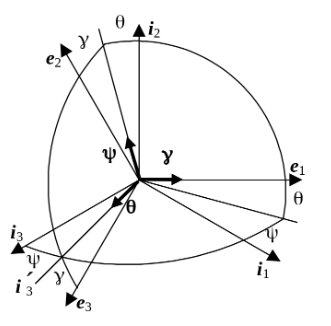
\includegraphics[width=0.6\linewidth]{krilov}
		\caption{Последовательность углов поворота Крылова ($i$ исходный базис, $e$ конечный)}
	\end{figure}
	1 поворот на угол рысканья $\psi$ вокруг оси $i_2$\\
	
	2 поворот на угол тангажа $\theta$ вокруг оси $i_3'$\\
	
	3 поворот на угол крена $\gamma$ вокруг оси $e_1$\\
	
	\addvspace{20pt}
	
	$A_\psi=\left[\begin{array}{ccc}\cos \psi & 0 & \sin \psi \\ 0 & 1 & 0 \\ -\sin \psi & 0 & \cos \psi\end{array}\right] A_\theta=\left[\begin{array}{ccc} \cos\gamma & -\sin \theta & 0 \\ \sin \theta & \cos \theta & 0 \\ 0 & 0 & 1\end{array}\right] A_\gamma=\left[\begin{array}{ccc}1 & 0 & 0 \\ 0 & \cos \gamma & -\sin \gamma \\ 0 & \sin \gamma & \cos \gamma\end{array}\right]$ \\
	
	\addvspace{20pt}

	$ A=A_\gamma A_\theta A_\psi=\left[\begin{array}{ccc}\cos \psi \cos \theta & -\cos \psi \sin \theta \cos \gamma+ \sin \psi \sin \gamma & \sin \gamma \cos \psi \sin \theta+ \sin \psi \cos \gamma \\ \sin \theta & \cos \theta \cos \gamma & \cos \theta \sin \gamma \\ -\sin \psi \cos \theta & \cos \gamma \sin \psi \sin \theta+ \cos \psi \sin \gamma & -\sin \gamma \sin \psi \sin \theta+ \cos \theta \cos_\gamma\end{array}\right]$
	
	
	
	
	
	
	
	
	
	
	
	
	
\end{document}